\documentclass[journal]{IEEEtran}
% ============================================================================
% SAGE-IDS — IEEE Transactions-style manuscript.
% Compile: pdflatex sage_ids ; bibtex sage_ids ; pdflatex sage_ids ; pdflatex sage_ids
% Figures in ./figures are produced by paper/make_figures.py from committed result JSON.
% Every quantitative value is cross-referenced to a file under reports/ in the repository.
% ============================================================================
\usepackage{cite}
\usepackage{amsmath,amssymb}
\usepackage{graphicx}
\usepackage{booktabs}
\usepackage{array}
\usepackage{xcolor}
\usepackage{url}
\usepackage[hidelinks]{hyperref}
\usepackage{tikz}
\usetikzlibrary{arrows.meta,positioning,shapes.geometric,fit,backgrounds}
\usepackage{algorithm}
\usepackage{algpseudocode}

\newcommand{\sage}{SAGE-IDS}
\newcommand{\code}[1]{\texttt{\small #1}}

\begin{document}

\title{\sage{}: Evidence-Gated Self-Evolving Intrusion Detection via\\
Closed-Loop Multi-Agent Adversarial Validation}

\author{Anand~Rawat,
        Anandi~Singh,
        Ananya~Agarwal,
        Brijesh~Kumar~Chaurasia,
        and~Ashutosh~Pandey%
\thanks{A. Rawat, A. Singh, and A. Agarwal are with the Department of Computer Science and
Engineering, Pranveer Singh Institute of Technology (PSIT), India
(e-mail: anandrawat138a@gmail.com).}%
\thanks{B. K. Chaurasia is with the Department of Mathematical Sciences and Computer Applications,
Bundelkhand University, Jhansi, Uttar Pradesh, India, and also with Pranveer Singh Institute of
Technology (PSIT), India (ORCID: 0000-0003-3708-7819).}%
\thanks{A. Pandey is with Pranveer Singh Institute of Technology (PSIT), India.}%
\thanks{Corresponding author: A. Rawat.}%
\thanks{Code, data manifests, and the full audit ledger are available at
\url{https://github.com/AnandRawat138/SAGE_IDS} (see Data Availability).}}

\markboth{Manuscript Preprint, November 2026}%
{Rawat \MakeLowercase{\textit{et al.}}: \sage{}: Evidence-Gated Self-Evolving Intrusion Detection}

\maketitle

\begin{abstract}
Intrusion-detection systems (IDS) are typically evaluated once, offline, and updated by hand.
Proposals to make detection ``self-evolving'' risk the opposite failure: an automated loop that
attacks, retrains, and deploys without control, and that can be gamed by its own feedback. We present
\sage{}, a multi-agent system in which a detector may change \emph{only} through an evidence-gated,
operator-approved protocol. Five agents---monitoring, threat research, adversarial validation,
remediation, and explanation---are driven by a persistent, bounded state machine. For every proposed
change, acceptance criteria are \emph{derived from a measured baseline, frozen, and cryptographically
committed before any candidate is evaluated}; candidates are compared against the current detector on
identical traffic with a paired exact test and gated on regression, false-positive, and
service-impact bounds. Each adversarial trial records three outcomes separately---executed, security
effect achieved, detected---so detection is never conflated with prevention. On a controlled
laboratory with real loopback packet capture and live NVD/MITRE ATT\&CK threat intelligence, the
protocol (i)~accepts changes that raise held-out detection F\textsubscript{1} from $0.54$ to $0.97$ at
zero measured false positives, (ii)~\emph{rejects} a plausible but over-sensitive change, and
(iii)~resists a feedback-poisoning shortcut (naive self-training) that a naive design would adopt.
A dedicated robustness study shows the accepted detectors are evadable by low-and-slow and
distributed variants, which we report as an explicit bound. A locally hosted large language model is
confined to a closed action set; on 30 live findings it agreed with the reviewed mapper $97\%$ of the
time and never exceeded that set. All artifacts, seeds, dataset hashes, and a hash-chained audit
ledger are released.
\end{abstract}

\begin{IEEEkeywords}
Intrusion detection, multi-agent systems, adversarial validation, closed-loop evaluation,
machine-learning security, reproducibility, large language models.
\end{IEEEkeywords}

% ===========================================================================
\section{Introduction}
\IEEEPARstart{N}{etwork} intrusion detection has been studied for decades, from signature engines such
as Snort~\cite{roesch1999snort} and Bro/Zeek~\cite{paxson1999bro} to a large body of machine-learning
(ML) detectors surveyed in~\cite{buczak2016survey}. Yet a persistent gap separates research from
practice. Sommer and Paxson~\cite{sommer2010closed} argued that intrusion detection differs from other
ML domains in the cost of errors, the semantic gap between anomalies and attacks, and the difficulty
of sound evaluation; many of their cautions remain unaddressed. ML-NIDS research continues to lean on
datasets---KDD'99 and its cleaned successor NSL-KDD~\cite{tavallaee2009nslkdd},
UNSW-NB15~\cite{moustafa2015unsw}, and CICIDS2017~\cite{sharafaldin2018cicids}---that are known to
contain duplicates, label noise, and feature-extraction faults~\cite{engelen2021troubleshooting}, and
on random train/test splits that overstate generalisation to unseen attacks, a bias formalised by
Pendlebury \emph{et al.}~\cite{pendlebury2019tesseract}.

A second gap concerns \emph{adaptation}. Detectors based on random forests~\cite{breiman2001random},
isolation forests~\cite{liu2008isolation}, autoencoder ensembles~\cite{mirsky2018kitsune}, or deep
sequence models~\cite{du2017deeplog} are usually trained once; when traffic drifts, they are retrained
manually. Work on concept-drift-robust NIDS~\cite{andresini2021insomnia} updates models
automatically, but automated adaptation introduces its own hazards: an attacker who influences the
feedback can poison the model, and adaptation under adversarial pressure is exactly where ML is
weakest~\cite{biggio2018wild,goodfellow2015adversarial}. Meanwhile, offensive tooling has become
highly automated---adversary emulation platforms such as CALDERA~\cite{applebaum2016caldera} generate
attacks from the MITRE ATT\&CK knowledge base~\cite{strom2018attack}---and large language models
(LLMs) are increasingly proposed for security operations~\cite{zhang2025llm}, raising the question of
how to use such automation \emph{safely} inside a defensive loop.

The phrase ``self-evolving defence'' therefore names a real need and a real danger. The need is to
close the loop: detect, validate against realistic attacks, improve, and re-validate. The danger is
that a naive closed loop becomes an unaccountable one---exploiting, retraining, and deploying without
evidence, review, or bounds, and confusing \emph{detecting} an attack with \emph{preventing} it. We
argue that the contribution worth making is not another adaptive model but a \emph{validation
discipline}: a protocol under which an IDS may evolve only when the evidence meets criteria that were
fixed in advance, and only with a human in the loop.

We present \sage{} (Self-evolving cyber defence through closed-loop multi-agent Adversarial validation
and adaptive intrusion detection). Its contributions are:

\begin{enumerate}
\item \textbf{An evidence-gated self-evolution protocol.} Acceptance criteria are derived from a
measured baseline, frozen, and committed to a hash-chained ledger \emph{before} any candidate is
tested; candidates are compared on identical traffic using a paired exact
test~\cite{dietterich1998tests} with interval estimates~\cite{wilson1927interval}, and activation
requires operator approval. ``Self-evolving'' thus means controlled, versioned, auditable change.
\item \textbf{A tri-outcome adversarial ledger} that records, per trial and separately, whether an
attack executed, achieved its security effect, and was detected---so a fix that prevents without
detecting, or detects without preventing, is visible rather than hidden.
\item \textbf{A feedback-poisoning control.} Retraining uses only labels verified by construction; we
quantify, as an ablation on identical data, how a naive self-training loop fails.
\item \textbf{A safety architecture for offensive-capable automation}: in-code target allowlists
enforced at every connection, opt-in active testing, LLM outputs confined to a closed reviewed action
set, and a tamper-evident ledger, with a documented threat model.
\item \textbf{An open, reproducible evaluation} on a real packet-capture laboratory, a live
threat-intelligence run, an evasion study, an LLM-vs-deterministic study, a leakage-controlled
CICIDS2017 benchmark, and multi-seed repetition, with every number traceable to a released artifact.
\end{enumerate}

% ===========================================================================
\section{Related Work and Positioning}
\label{sec:related}
\textbf{Signature and anomaly NIDS.} Snort~\cite{roesch1999snort} and Bro/Zeek~\cite{paxson1999bro}
established rule- and policy-based detection; ML-based anomaly detection is surveyed
in~\cite{buczak2016survey}, with representative systems using isolation
forests~\cite{liu2008isolation}, autoencoder ensembles~\cite{mirsky2018kitsune}, and deep sequence
models~\cite{du2017deeplog}. These target \emph{what} to detect; \sage{} is orthogonal---it governs
\emph{when and how} a detector is allowed to change.

\textbf{Evaluation methodology.} Sommer and Paxson~\cite{sommer2010closed} catalogued why ML-NIDS
evaluation is hard. Dataset critiques~\cite{tavallaee2009nslkdd,engelen2021troubleshooting} and the
space/time-bias framework of TESSERACT~\cite{pendlebury2019tesseract} show that common protocols
inflate results. We adopt dedup-before-split, train-only preprocessing, and an unseen-day split, and
reproduce the optimism gap (Sec.~\ref{sec:benchmark}); we extend this discipline from offline datasets
to an online closed loop with pre-committed acceptance criteria.

\textbf{Adaptive and drift-robust NIDS.} Online detectors~\cite{mirsky2018kitsune,du2017deeplog} and
concept-drift-robust systems such as INSOMNIA~\cite{andresini2021insomnia} update models as traffic
changes. They do not pre-register acceptance criteria, do not separate prevention from detection, and
do not place a human gate before activation---precisely the controls \sage{} adds.

\textbf{Adversary emulation and LLM agents.} CALDERA~\cite{applebaum2016caldera} automates ATT\&CK-based
attacks~\cite{strom2018attack}; LLMs are increasingly applied to security
tasks~\cite{zhang2025llm}. \sage{} uses bounded, reviewed emulation inside a validation loop and
confines the LLM to selecting from a closed, auditable action set, measuring rather than trusting it.

\textbf{Adversarial ML.} Evasion and poisoning~\cite{biggio2018wild,goodfellow2015adversarial} motivate
our verified-label constraint and our explicit evasion study (Sec.~\ref{sec:evasion}).

Table~\ref{tab:related} positions \sage{} against representative lines of work along the axes that
define our contribution.

\begin{table*}[t]
\caption{Positioning of \sage{} against representative work. ``Closed loop'' = attacks feed back into
validated detector change; ``pre-committed criteria'' = acceptance thresholds fixed before evaluating
candidates; ``prevention $\neq$ detection'' = the two outcomes are measured separately; ``poisoning
control'' = learning restricted to verified labels; ``operator gate'' = human approval before
activation; ``audit'' = tamper-evident provenance.}
\label{tab:related}
\centering
\small
\begin{tabular}{@{}lccccccc@{}}
\toprule
System / line of work & Closed loop & Adversarial & Pre-committed & Prevention & Poisoning & Operator & Tamper-evident \\
 & & validation & criteria & $\neq$ detection & control & gate & audit \\
\midrule
Signature IDS~\cite{roesch1999snort,paxson1999bro}        & -- & -- & -- & -- & n/a & manual & -- \\
ML-NIDS surveys~\cite{buczak2016survey}                    & -- & -- & -- & -- & -- & -- & -- \\
Online/anomaly~\cite{mirsky2018kitsune,du2017deeplog}      & partial & -- & -- & -- & -- & -- & -- \\
Drift-robust (INSOMNIA)~\cite{andresini2021insomnia}       & yes & -- & -- & -- & partial & -- & -- \\
Adversary emulation~\cite{applebaum2016caldera}            & -- & yes & -- & -- & n/a & manual & -- \\
Eval frameworks~\cite{pendlebury2019tesseract}             & -- & -- & yes (offline) & -- & -- & n/a & -- \\
\textbf{\sage{} (this work)}                               & \textbf{yes} & \textbf{yes} & \textbf{yes} & \textbf{yes} & \textbf{yes} & \textbf{yes} & \textbf{yes} \\
\bottomrule
\end{tabular}
\end{table*}

% ===========================================================================
\section{System Design}
\label{sec:design}

\begin{figure*}[t]
\centering
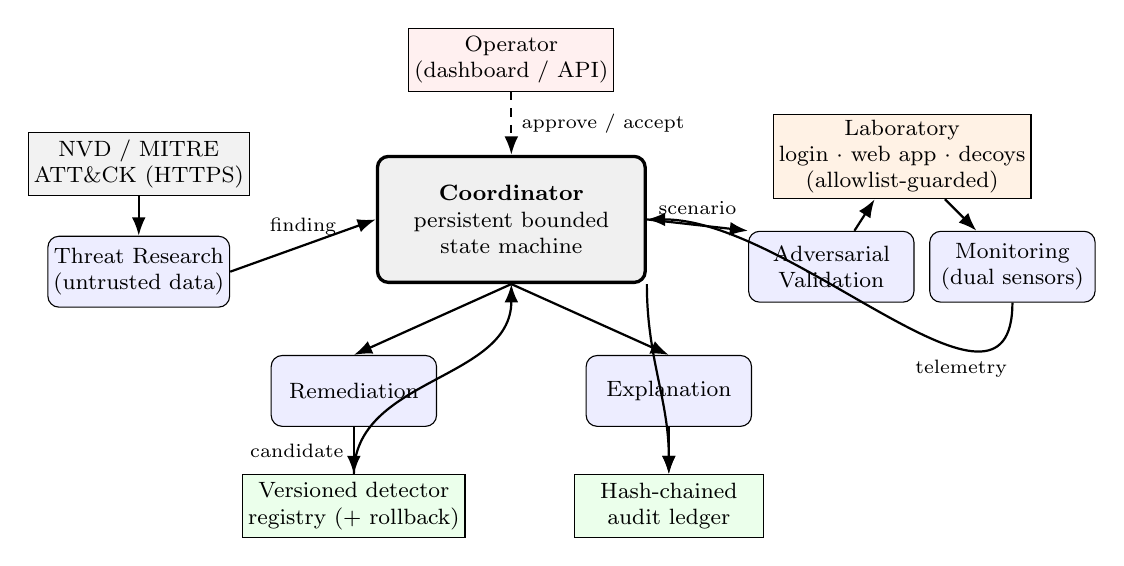
\begin{tikzpicture}[>=Latex, font=\footnotesize, node distance=6mm and 10mm,
  agent/.style={draw, rounded corners, align=center, minimum width=21mm, minimum height=9mm,
    fill=blue!7, inner sep=2pt},
  core/.style={draw, very thick, rounded corners, align=center, minimum width=34mm,
    minimum height=16mm, fill=gray!12},
  store/.style={draw, align=center, minimum width=24mm, minimum height=8mm, fill=green!8,
    inner sep=2pt},
  lab/.style={draw, align=center, minimum width=26mm, minimum height=9mm, fill=orange!10,
    inner sep=2pt},
  ext/.style={draw, align=center, minimum width=20mm, minimum height=8mm, fill=black!5,
    inner sep=2pt},
  op/.style={draw, align=center, minimum width=22mm, minimum height=8mm, fill=red!6, inner sep=2pt},
  dat/.style={->, thick}, ctl/.style={->, thick, dashed}]
% centre: coordinator
\node[core] (co) {\textbf{Coordinator}\\persistent bounded\\state machine};
% operator above
\node[op, above=8mm of co] (op) {Operator\\(dashboard / API)};
% left: threat intelligence
\node[ext, left=16mm of co, yshift=7mm] (nvd) {NVD / MITRE\\ATT\&CK (HTTPS)};
\node[agent, below=5mm of nvd] (tr) {Threat Research\\(untrusted data)};
% right: lab + its two agents
\node[lab, right=16mm of co, yshift=8mm] (lab) {Laboratory\\login $\cdot$ web app $\cdot$ decoys\\(allowlist-guarded)};
\node[agent, below=4mm of lab, xshift=-9mm] (adv) {Adversarial\\Validation};
\node[agent, below=4mm of lab, xshift=14mm] (mon) {Monitoring\\(dual sensors)};
% below coordinator: remediation + explanation
\node[agent, below=9mm of co, xshift=-20mm] (rem) {Remediation};
\node[agent, below=9mm of co, xshift=20mm] (exp) {Explanation};
% bottom stores
\node[store, below=6mm of rem] (reg) {Versioned detector\\registry (+ rollback)};
\node[store, below=6mm of exp] (led) {Hash-chained\\audit ledger};
% edges: data plane (solid), control/approval (dashed)
\draw[dat] (nvd) -- (tr);
\draw[dat] (tr.east) -- node[above, font=\scriptsize]{finding} (co.west);
\draw[ctl] (op) -- node[right, font=\scriptsize]{approve / accept} (co);
\draw[dat] (co.east) -- node[above, font=\scriptsize]{scenario} (adv.north west);
\draw[dat] (adv) -- (lab);
\draw[dat] (lab) -- (mon);
\draw[dat] (mon.south) to[out=-90,in=0] node[below, font=\scriptsize, pos=0.3]{telemetry} (co.east);
\draw[dat] (co.south) -- (rem.north);
\draw[dat] (co.south) -- (exp.north);
\draw[dat] (rem) -- node[left, font=\scriptsize]{candidate} (reg);
\draw[dat] (reg.north) to[out=90,in=-90] (co.south);
\draw[dat] (exp) -- (led);
\draw[dat] (co.south east) to[out=-90,in=90] (led.north);
\end{tikzpicture}
\caption{\sage{} architecture. Solid arrows are the data plane; dashed arrows are the
operator control plane. Retrieved intelligence is untrusted and never executed; the Adversarial
Validation agent reaches the laboratory only through an in-code target allowlist; every coordinator
transition and detector-version change is written to the hash-chained audit ledger. A candidate
version activates only via the operator after passing the frozen acceptance criteria.}
\label{fig:arch}
\end{figure*}

\subsection{Agents and coordinator}
\sage{} comprises five agents coordinated by a persistent, bounded state machine
(Fig.~\ref{fig:fsm}; the overall architecture is shown in Fig.~\ref{fig:arch}). The \emph{Monitoring}
agent ingests telemetry, builds per-source feature
windows, attaches ground-truth labels, and runs the active detector. The \emph{Threat Research} agent
retrieves vulnerability and technique intelligence (Sec.~\ref{sec:intel}). The \emph{Adversarial
Validation} agent executes reviewed scenarios against allowlisted laboratory targets. The
\emph{Remediation} agent proposes bounded defensive changes. The \emph{Explanation} agent produces
evidence-grounded reports. Transitions are role-checked (system vs.\ operator), recorded with their
evidence, and appended to a SHA-256 hash-chained ledger; running phases are claimed with an atomic
compare-and-set so no phase executes twice; retries and adaptation cycles are bounded; and stale runs
time out on restart rather than silently resuming.

\begin{figure}[t]
\centering
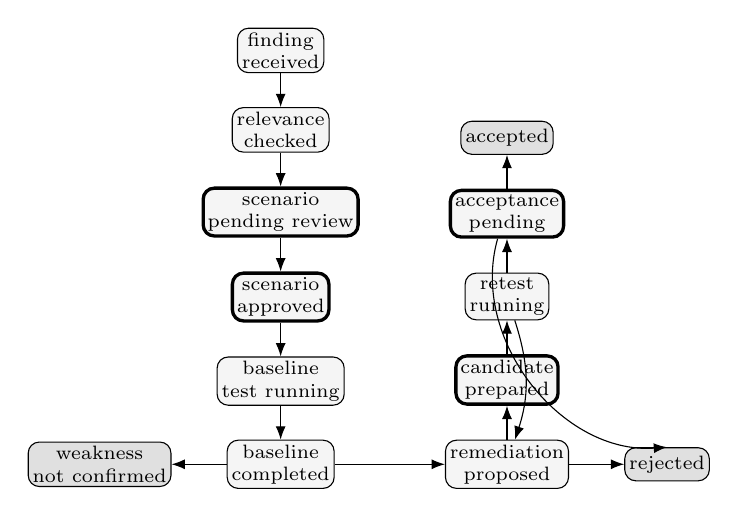
\begin{tikzpicture}[>=Latex, node distance=4.3mm and 6mm,
  every node/.style={font=\scriptsize},
  st/.style={draw, rounded corners, align=center, inner sep=1.6pt, minimum height=4.2mm, fill=gray!8},
  term/.style={st, fill=black!12},
  op/.style={draw=black, very thick}]
\node[st] (fr) {finding\\received};
\node[st, below=of fr] (rc) {relevance\\checked};
\node[st, below=of rc, op] (pr) {scenario\\pending review};
\node[st, below=of pr, op] (ap) {scenario\\approved};
\node[st, below=of ap] (bt) {baseline\\test running};
\node[st, below=of bt] (bc) {baseline\\completed};
\node[st, right=14mm of bc] (rp) {remediation\\proposed};
\node[st, above=of rp, op] (cp) {candidate\\prepared};
\node[st, above=of cp] (rt) {retest\\running};
\node[st, above=of rt, op] (acp) {acceptance\\pending};
\node[term, above=of acp] (acc) {accepted};
\node[term, right=7mm of rp] (rej) {rejected};
\node[term, left=7mm of bc] (wnc) {weakness\\not confirmed};
\draw[->] (fr)--(rc); \draw[->] (rc)--(pr); \draw[->] (pr)--(ap);
\draw[->] (ap)--(bt); \draw[->] (bt)--(bc);
\draw[->] (bc)--(rp); \draw[->] (bc)--(wnc);
\draw[->] (rp)--(cp); \draw[->] (cp)--(rt); \draw[->] (rt)--(acp);
\draw[->] (acp)--(acc);
\draw[->] (rt) to[bend left=18] (rp);
\draw[->] (rp)--(rej); \draw[->] (acp) to[bend right=55] (rej.north);
\end{tikzpicture}
\caption{Coordinator state machine (bold = operator-gated transition; shaded = terminal). Additional
terminal states \code{not\_relevant}, \code{inconclusive}, \code{failed}, \code{cancelled}, and
\code{timed\_out} are omitted for clarity. Each transition is validated, recorded with evidence, and
hash-chained.}
\label{fig:fsm}
\end{figure}

\subsection{Laboratory and dual sensors}
The laboratory consists of loopback services---a dummy login endpoint, a test web application, and
decoy listeners---bound to localhost. Two sensors observe them. An application-level sensor records
request/response metadata. A \emph{real packet-capture sensor} (built on a user-space capture driver)
sniffs loopback TCP, assembles bidirectional flows, and derives flow statistics in a
CICIDS2017-compatible schema; unlike the application sensor it observes SYN/RST exchanges to closed
ports, giving packet-faithful reconnaissance telemetry. An isolated container variant with Zeek and
Suricata is provided as a deployment template.

\subsection{Detection and versioning}
A detector \emph{version} bundles threshold rules, a random forest~\cite{breiman2001random} (with an
optional isolation forest~\cite{liu2008isolation} in shadow mode), the laboratory configuration, the
feature-schema hash, and the label-set digest, all hashed together. Versions are
candidate/accepted/retired; activation requires a human operator and a passed evaluation; rollback
re-activates a previous accepted version. Rules are evaluated online over per-source sliding windows,
yielding a detection latency as well as a decision.

\subsection{Threat intelligence as untrusted data}
\label{sec:intel}
The Threat Research agent retrieves CVE records from NVD and techniques from MITRE
ATT\&CK~\cite{strom2018attack} over HTTPS, with host allowlisting, timeouts, caching, rate limiting,
provenance capture, and deduplication. Retrieved text is treated as untrusted: it is sanitised,
length-limited, scanned for instruction-like content, stored, and \emph{never executed}. Findings are
mapped to reviewed scenarios deterministically by weakness class (CWE) and technique. An optional
LLM may corroborate the mapping but is confined to selecting identifiers from the closed allowed set
(Sec.~\ref{sec:llm}).

\subsection{Evidence-gated acceptance}
\label{sec:accept}
After the baseline test, numeric criteria are derived from the measured baseline, frozen, and
hash-committed before any candidate is evaluated. The objective depends on the confirmed weakness:
a \emph{detection} objective (paired McNemar gain~\cite{dietterich1998tests}, Wilson lower
bound~\cite{wilson1927interval}, and ``effect not increased'') or a \emph{prevention} objective
(effect-rate reduction, one-sided Fisher test, and ``detection non-inferior''), plus a
regression-non-inferiority bound over previously passed scenarios, a benign false-positive bound, and
a service-health check. All candidates of a case are retested under common random seeds; the held-out
final test uses a disjoint seed range. Algorithm~\ref{alg:loop} summarises one cycle.

\begin{algorithm}[t]
\caption{One evidence-gated adaptation cycle}
\label{alg:loop}
\begin{algorithmic}[1]
\State finding $\gets$ ThreatResearch(); scenario $\gets$ map(finding) \Comment{closed set}
\State \textbf{require} operator approval of scenario
\State $B \gets$ BaselineTest(scenario, active version) \Comment{exec/effect/detect per trial}
\State \textbf{if} weakness not confirmed \textbf{then} report; \textbf{return}
\State $C \gets$ DeriveCriteria($B$); commit $\mathrm{SHA\text{-}256}(C)$ to ledger
\For{proposal in Remediation($B$)}
  \State $v \gets$ PrepareCandidate(proposal) \Comment{verified labels only}
  \State $R \gets$ Retest($v$, common seeds) \Comment{paired with baseline}
  \State \textbf{if} Evaluate($C, R$) passes \textbf{and} operator accepts
  \State \quad \textbf{then} activate($v$); \textbf{break}
\EndFor
\State Explain(evidence); \textbf{rollback} available
\end{algorithmic}
\end{algorithm}

% ===========================================================================
\section{Threat Model and Safety}
\label{sec:threat}
\sage{} contains offensive-capable components, so its primary risk is being turned against unintended
targets or being gamed through its feedback. We summarise controls; the full model is released.

\emph{Target confinement.} A CIDR+port allowlist is enforced in code at scenario selection and again at
every socket connection (hostname resolution, connected-peer re-check, source-range check); active
scenarios are opt-in. \emph{Untrusted intelligence.} Retrieved content is sanitised and never executed;
the deterministic CWE/technique mapping, not the content, drives actions. \emph{LLM confinement.} LLM
output is schema-validated and intersected with the reviewed catalogue, so it can never widen the
action set, change a target, or alter a state (verified empirically in Sec.~\ref{sec:llm}).
\emph{Unsafe-deployment prevention.} A candidate activates only after a passed evaluation against
pre-committed criteria and explicit operator approval; there is no production path. \emph{Integrity.}
Model bundles carry SHA-256 digests checked on load; the audit ledger is hash-chained and verified.
Residual risks---tamper-evident is not tamper-proof, loopback shares the host kernel, and the allowlist
trusts the resolver---are documented.

% ===========================================================================
\section{Evaluation}
\label{sec:eval}
Unless noted, each experiment phase uses 30 trials, Wilson 95\% intervals, and paired exact McNemar
tests; attacker and benign clients use distinct loopback source addresses, giving ground-truth labels
by construction. Environment: Python~3.12, scikit-learn~1.9, a 16-core host. Every figure and table is
regenerated from a released JSON artifact.

\subsection{Closed-loop case study}
\label{sec:casestudy}
Table~\ref{tab:cases} lists the outcomes of one clean run. Three cases exercise the protocol: a
detection weakness that is fixed (password guessing), a detection weakness fixed by retraining
(request flood), and a \emph{prevention} weakness that is correctly \emph{not} fixed by detection
(reconnaissance). A fourth finding carrying instruction-like injected text is flagged untrusted and
denied by the operator.

\begin{table}[t]
\caption{Closed-loop case outcomes (run \code{145253Z}). ``Baseline'' gives per-trial detection and
security-effect of the initial detector v1.}
\label{tab:cases}
\centering
\small
\begin{tabular}{@{}llll@{}}
\toprule
Case & Baseline (detect / effect) & Candidates & Outcome \\
\midrule
Password guessing & $0/30$ / $30/30$ & 2 (1 rejected) & accepted v3 \\
Request flood     & $0/30$ / $30/30$ & 1 & accepted v4 \\
Reconnaissance    & $30/30$ / $21/30$ & 2 & all rejected \\
Injected finding  & n/a & 0 & operator-denied \\
\bottomrule
\end{tabular}
\end{table}

For password guessing, a maximum-sensitivity rule is \emph{rejected} because it raises the benign
false-positive rate to $0.167$ against the frozen bound of $0.02$; a calibrated rule plus account
lockout is accepted. For reconnaissance, the baseline already detects every probe ($30/30$) but the
probe still achieves its effect ($21/30$); no detection-only candidate can satisfy a prevention
objective, so both candidates are rejected---a decision the tri-outcome ledger makes principled rather
than arbitrary. Fig.~\ref{fig:window} shows window-level F\textsubscript{1} and benign false-positive
rate across all versions produced in the run; Fig.~\ref{fig:detect} shows per-scenario detection of
the initial vs.\ accepted detectors on the held-out final test (fresh seeds, identical traffic): window
F\textsubscript{1} rises from $0.54$ to $0.97$ at $0/102$ benign false positives, flood detection from
$0/30$ to $30/30$, and password-guessing from $0/30$ to $27/30$ (the three misses succeed within
$\leq 3$ attempts and are behaviourally indistinguishable from user typos).

\begin{figure}[t]
\centering
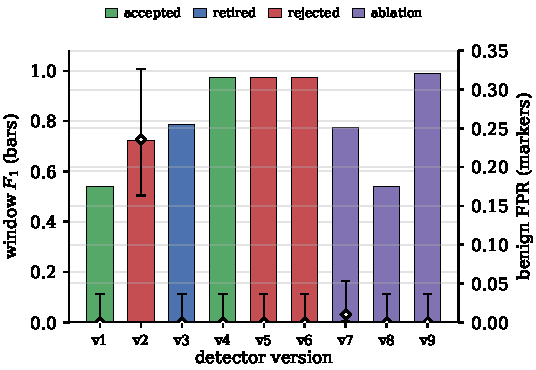
\includegraphics[width=0.84\columnwidth]{figures/fig_window_versions.pdf}
\caption{Held-out window-level F\textsubscript{1} (bars) and benign false-positive rate (line) for
each detector version in run \code{145253Z}. Rejected candidates (e.g.\ the high-FPR v2) never
activate.}
\label{fig:window}
\end{figure}

\begin{figure}[t]
\centering
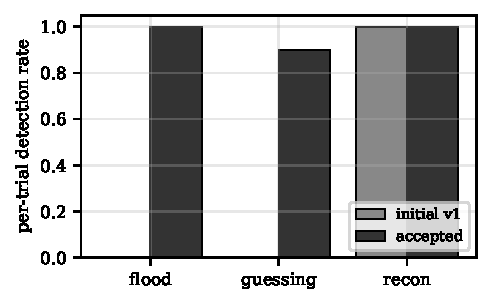
\includegraphics[width=0.84\columnwidth]{figures/fig_final_detection.pdf}
\caption{Per-scenario held-out detection rate: initial detector v1 vs.\ accepted versions, identical
traffic. Reconnaissance is already detected by v1; the gain is on guessing and flood.}
\label{fig:detect}
\end{figure}

Table~\ref{tab:accept} shows the frozen acceptance criteria and the pass/fail of each candidate,
read from the committed evaluation records. The screenshot in Fig.~\ref{fig:dash} shows the operator
dashboard exposing the committed criteria hash---the commitment a reviewer can verify against the
ledger.

\begin{table}[t]
\caption{Candidate evaluations against pre-committed criteria (run \code{145253Z}). Only passing
candidates with operator approval are activated.}
\label{tab:accept}
\centering
\small
\begin{tabular}{@{}lll@{}}
\toprule
Candidate & Objective & Result (binding check) \\
\midrule
v2 (max-sensitivity rule)      & detection  & \textbf{reject} (benign FPR $0.167>0.02$) \\
v3 (calibrated rule+lockout)   & detection  & \textbf{pass} \\
v4 (verified retrain)          & detection  & \textbf{pass} \\
v5 (recon rule)                & prevention & \textbf{reject} (effect not reduced) \\
v6 (recon retrain)             & prevention & \textbf{reject} (effect not reduced) \\
\bottomrule
\end{tabular}
\end{table}

\begin{figure}[t]
\centering
\fbox{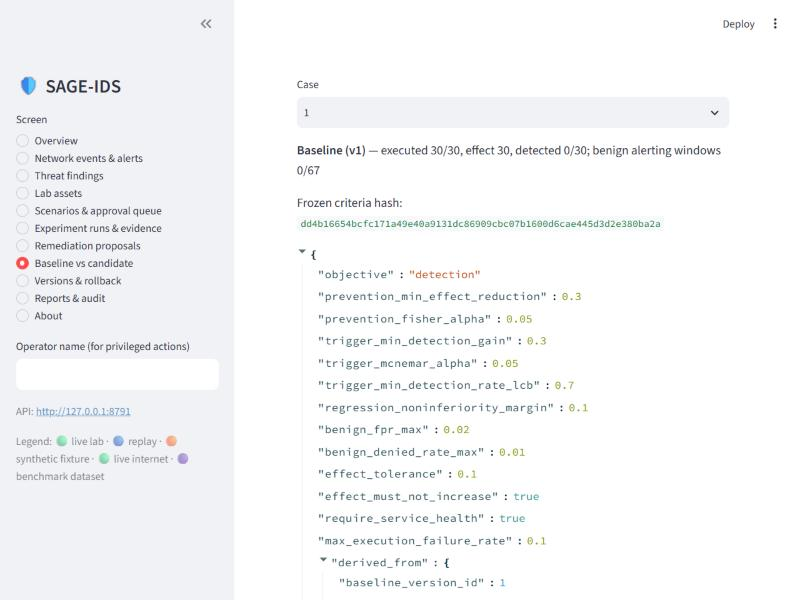
\includegraphics[width=0.92\columnwidth]{figures/screenshot_baseline_candidate.jpg}}
\caption{Operator dashboard (baseline-vs-candidate screen) showing the baseline measurement and the
\emph{frozen criteria hash} committed before any candidate was evaluated.}
\label{fig:dash}
\end{figure}

\subsection{Feedback-poisoning and static-baseline ablations}
\label{sec:ablation}
Two ablations use the same held-out traffic. \emph{Naive self-training}---retraining on pseudo-labels
from the current model---detects $0/30$ of both attacks, because a model cannot label attacks it
already misses; verified-label retraining detects $30/30$ of each. This is a direct, measured argument
for the verified-label constraint. \emph{Static baseline}---enabling the isolation forest on v1 with no
adaptation---reaches window F\textsubscript{1} $0.78$; we therefore report the adapted version's gain
over this stronger baseline (to $0.97$), not only over the initial rules.

\subsection{Robustness to evasion}
\label{sec:evasion}
We run reviewed evasive variants against the \emph{accepted} detectors (Fig.~\ref{fig:evasion}). The
accepted password-guessing detector falls from $27/30$ on the normal attack to $3/12$ (low-and-slow)
and $0/12$ (distributed, one source per attempt); the flood detector catches $9/12$ of a low-rate
flood. The accepted fixes are genuine improvements against the tested threat but are \emph{not} robust
defences---an honest bound that the protocol surfaces rather than conceals, consistent with the
adversarial-ML literature~\cite{biggio2018wild}.

\begin{figure}[t]
\centering
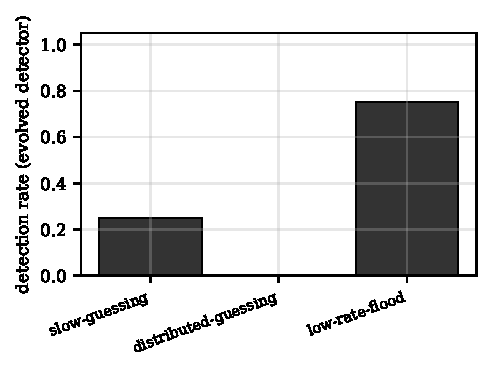
\includegraphics[width=0.84\columnwidth]{figures/fig_evasion.pdf}
\caption{Detection rate of the evolved detector against reviewed evasive variants. Each variant still
achieves its security effect; low detection indicates evadability of behavioural per-source thresholds.}
\label{fig:evasion}
\end{figure}

\subsection{Live threat intelligence and LLM confinement}
\label{sec:llm}
A live run retrieved 46 findings (40 NVD CVEs, 6 ATT\&CK techniques); 42 mapped to laboratory assets
by weakness class, yielding real cases from current intelligence. We then measured a locally hosted
LLM (Llama-3-8B) against the reviewed deterministic mapper. On 30 live findings the LLM produced
valid structured output $100\%$ of the time, independently selected the reviewed scenario $97\%$ of
the time at a mean latency of $2.75$\,s, and---by construction---\emph{never} selected outside the
closed allowed set. The LLM thus adds corroboration without widening the action space; even at $0\%$
agreement the system remains safe, because only the deterministic mapping and the operator drive
execution.

\subsection{Benchmark with leakage controls}
\label{sec:benchmark}
To place the detector family in context we benchmark on the full CICIDS2017
dataset~\cite{sharafaldin2018cicids} ($2{,}830{,}743$ flows; $2{,}496{,}544$ after
dedup-before-split; zero cross-split identical-row overlap on every seed), with train-only
preprocessing and validation-selected thresholds, over five seeds. Fig.~\ref{fig:bench} contrasts a
random stratified split (random forest F\textsubscript{1} $0.998$) with an unseen-day split (train
Mon--Thu, test Fri; F\textsubscript{1} $0.540$, recall $0.370$). The gap---more than $0.45$
F\textsubscript{1}---quantifies the optimism of random-split evaluation for unseen attack families,
reproducing the space/time-bias concern~\cite{pendlebury2019tesseract} on a network dataset and
motivating the unseen-attack posture of our closed loop.

\begin{figure}[t]
\centering
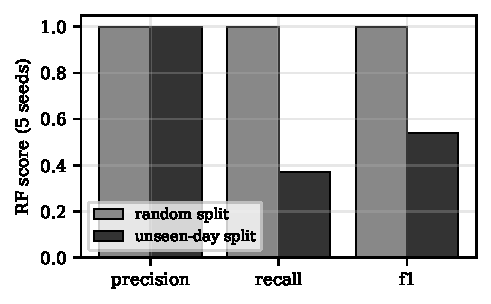
\includegraphics[width=0.84\columnwidth]{figures/fig_benchmark_split.pdf}
\caption{CICIDS2017 random-forest performance (5 seeds): random split vs.\ unseen-day split. High
recall collapses on attack families absent from training.}
\label{fig:bench}
\end{figure}

\subsection{Multi-seed stability}
\label{sec:multiseed}
To address single-realisation bias we repeat the full protocol under three independent base seeds
(attacker parameters, trial order, benign traffic, and model seeds all vary; Table~\ref{tab:multiseed}).
The accept/reject \emph{decisions are identical across all three seeds}---password guessing and request
flood accepted, reconnaissance rejected---and the held-out detection rates are tight: flood
$0.00\!\to\!1.00$, password guessing $0.00\!\to\!0.90$, reconnaissance $1.00\!\to\!1.00$ (mean over
seeds, $95\%$ bootstrap interval width $\leq 0.00$ at this precision). The protocol's outcomes are thus
not artifacts of one random draw. The automated timing-integrity check flagged one seed in which two
reconnaissance baseline trials ran abnormally long ($159$\,s and $317$\,s) under host CPU contention
(no inter-run gaps, i.e.\ not a host suspend); this inflates detection-latency on those two trials but
does not affect the logical executed/effect/detected outcomes or the decisions, which match the other
seeds exactly. We report it rather than suppress it, as an instance of the integrity check working.

\begin{table}[t]
\caption{Multi-seed stability (3 realisations). Case decisions are identical across seeds; held-out
per-scenario detection is mean over seeds.}
\label{tab:multiseed}
\centering
\small
\begin{tabular}{@{}lccc@{}}
\toprule
 & seed 1 & seed 2 & seed 3 \\
\midrule
Password guessing & accept & accept & accept \\
Request flood     & accept & accept & accept \\
Reconnaissance    & reject & reject & reject \\
\midrule
 & \multicolumn{3}{c}{detection: initial v1 $\to$ accepted (mean)} \\
\midrule
flood             & \multicolumn{3}{c}{$0.00 \to 1.00$} \\
password guessing & \multicolumn{3}{c}{$0.00 \to 0.90$} \\
reconnaissance    & \multicolumn{3}{c}{$1.00 \to 1.00$} \\
\bottomrule
\end{tabular}
\end{table}

\subsection{Cost and auditability}
Detector inference costs on the order of $1$\,ms per feature window; one full closed-loop run
(bootstrap, three cases, ablations, held-out test) completes in under $20$ minutes on the 16-core
host at $\approx 250$\,MB resident memory. The run's hash-chained ledger verifies intact, and a
tamper test that modifies one ledger entry on a copy is detected at that entry---evidence integrity is
mechanically checkable.

% ===========================================================================
\section{Discussion and Limitations}
\label{sec:limits}
\sage{}'s results are laboratory results. Targets are loopback services; benign traffic is synthetic;
the scenario set is small. The operator is scripted in the reported runs, so the human gate is
exercised mechanically rather than by independent judgement. The accepted fixes are evadable
(Sec.~\ref{sec:evasion}). The benchmark uses one dataset with known label
issues~\cite{engelen2021troubleshooting}. The audit ledger is tamper-evident, not externally anchored.
These bounds are stated so that the protocol's guarantees---pre-commitment, paired testing,
tri-outcome accounting, verified-label learning, and operator approval---are not over-read. The design
transfers directly to a packet-capture testbed with real services, which we provide as a container
template; doing so, and adding evasive and multi-source scenarios to the approved catalogue, is the
natural next step.

% ===========================================================================
\section{Data Availability}
The complete source code, configuration, synthetic fixtures, dataset SHA-256 manifests, model cards,
per-run result JSON, generated reports, and the full hash-chained audit ledger are available at
\url{https://github.com/AnandRawat138/SAGE_IDS}. The CICIDS2017~\cite{sharafaldin2018cicids} and
UNSW-NB15~\cite{moustafa2015unsw} datasets are obtained from their original providers under their
respective terms; we release only file hashes and preprocessing code, not the data. Every quantitative
claim in this paper is reproduced by the commands in the repository's reproducibility guide.

% ===========================================================================
\section{Conclusion}
\sage{} reframes ``self-evolving defence'' as an auditable, evidence-gated protocol rather than
autonomous adaptation. A detector may change only when pre-committed criteria are met on identical
traffic under a paired test, learning is restricted to verified labels, and an operator approves the
change; detection and prevention are measured separately throughout. On a real packet-capture
laboratory with live intelligence, the protocol accepts genuine improvements, rejects an
over-sensitive change and a mis-targeted one, resists a feedback-poisoning shortcut, and reports its
own evadability. The contribution is the validation discipline and an honest, reproducible measurement
of what such a loop does and does not achieve.

\section*{Acknowledgment}
This work used only locally hosted models and public threat-intelligence feeds. The authors thank
their institutions for infrastructure support.

\bibliographystyle{IEEEtran}
\bibliography{refs}

\end{document}
